\section{Centroid Alignment} \label{sec:Centroid_Alignment}

\blindtext

\begin{figure}[!hbt]
    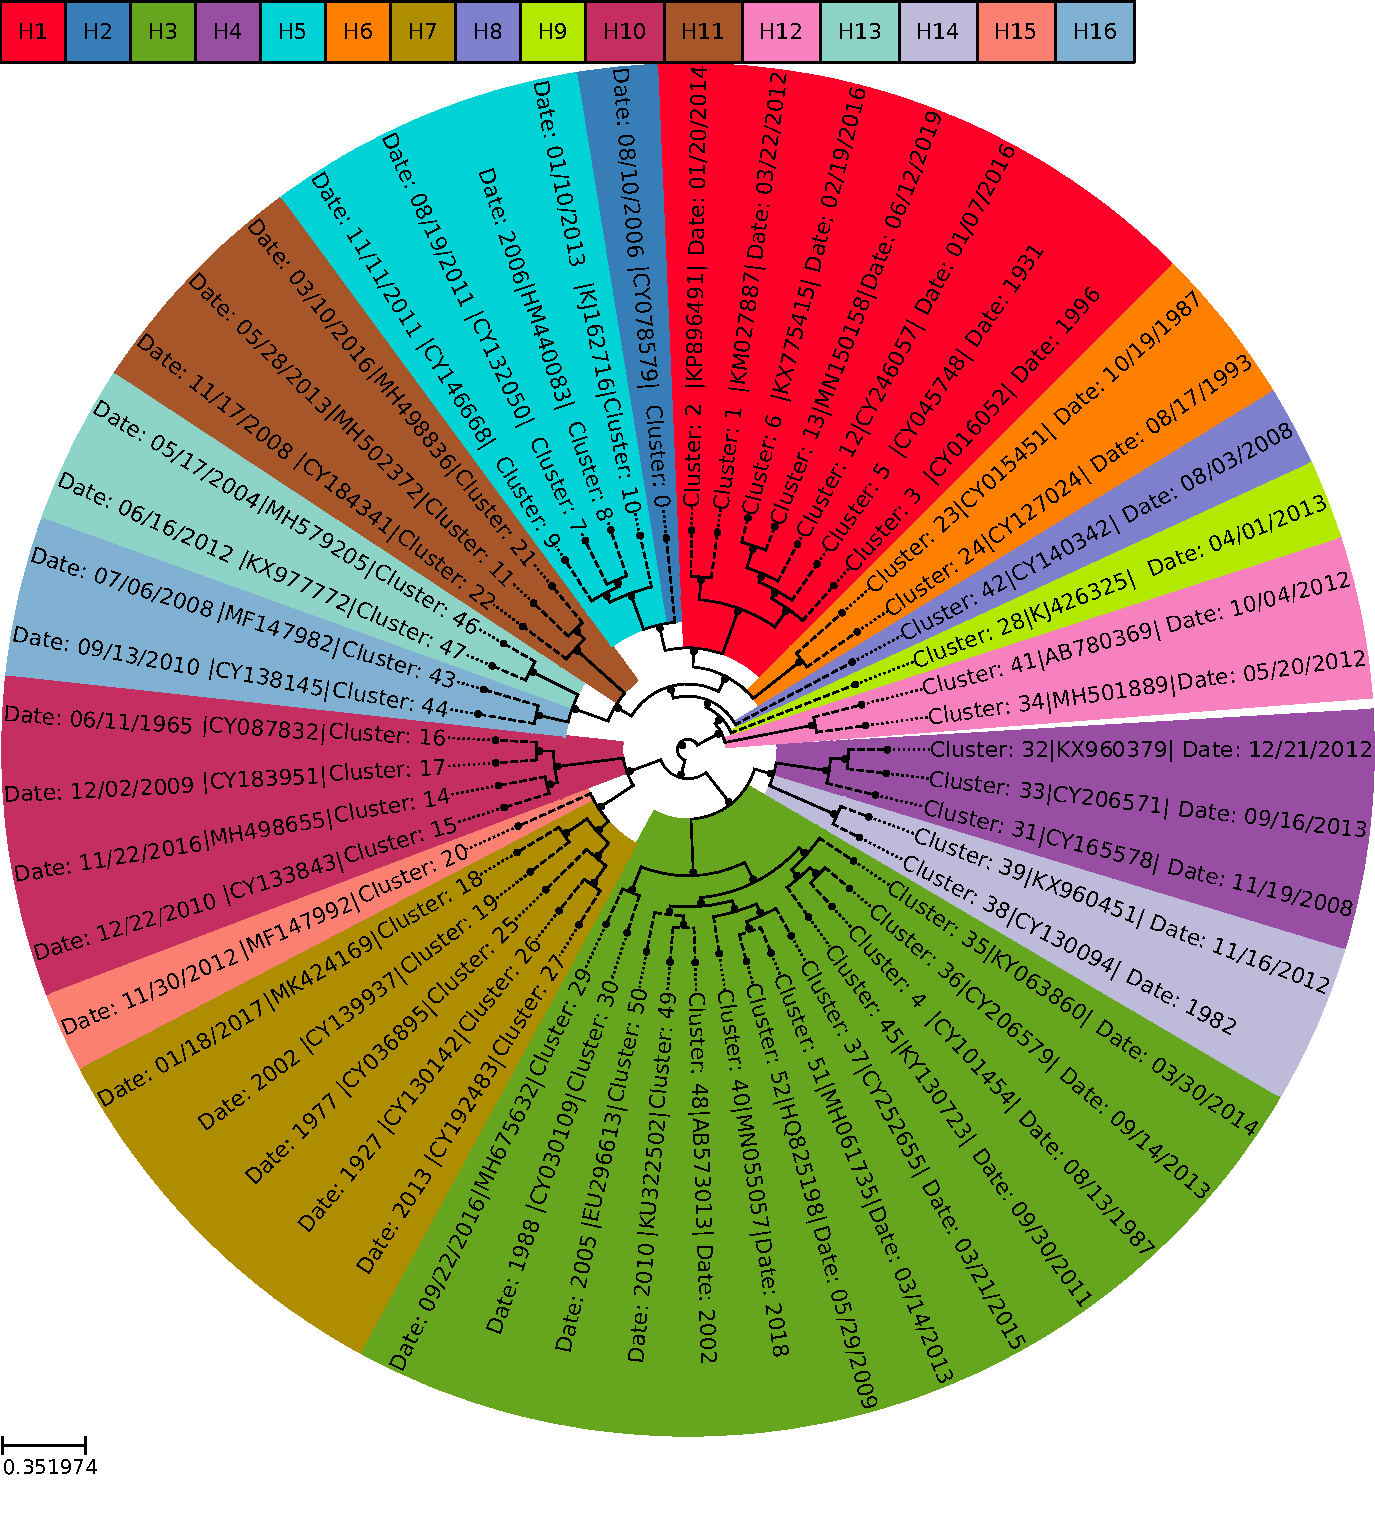
\includegraphics[width=\dimexpr\textwidth-2\fboxsep-2\fboxrule,fbox]{PCA/Guidetree_segment_4_H_Centroid.pdf}
    \caption[Knee based Segment 4 Guidetree with \Acrshort{PCA}]{\textbf{Knee based Segment 4 Guidetree with \Acrshort{PCA}.} .}
    \label{fig:PCA_Guidetree_Centroid_4}
\end{figure}

\blindtext

\begin{figure}[!hbt]
    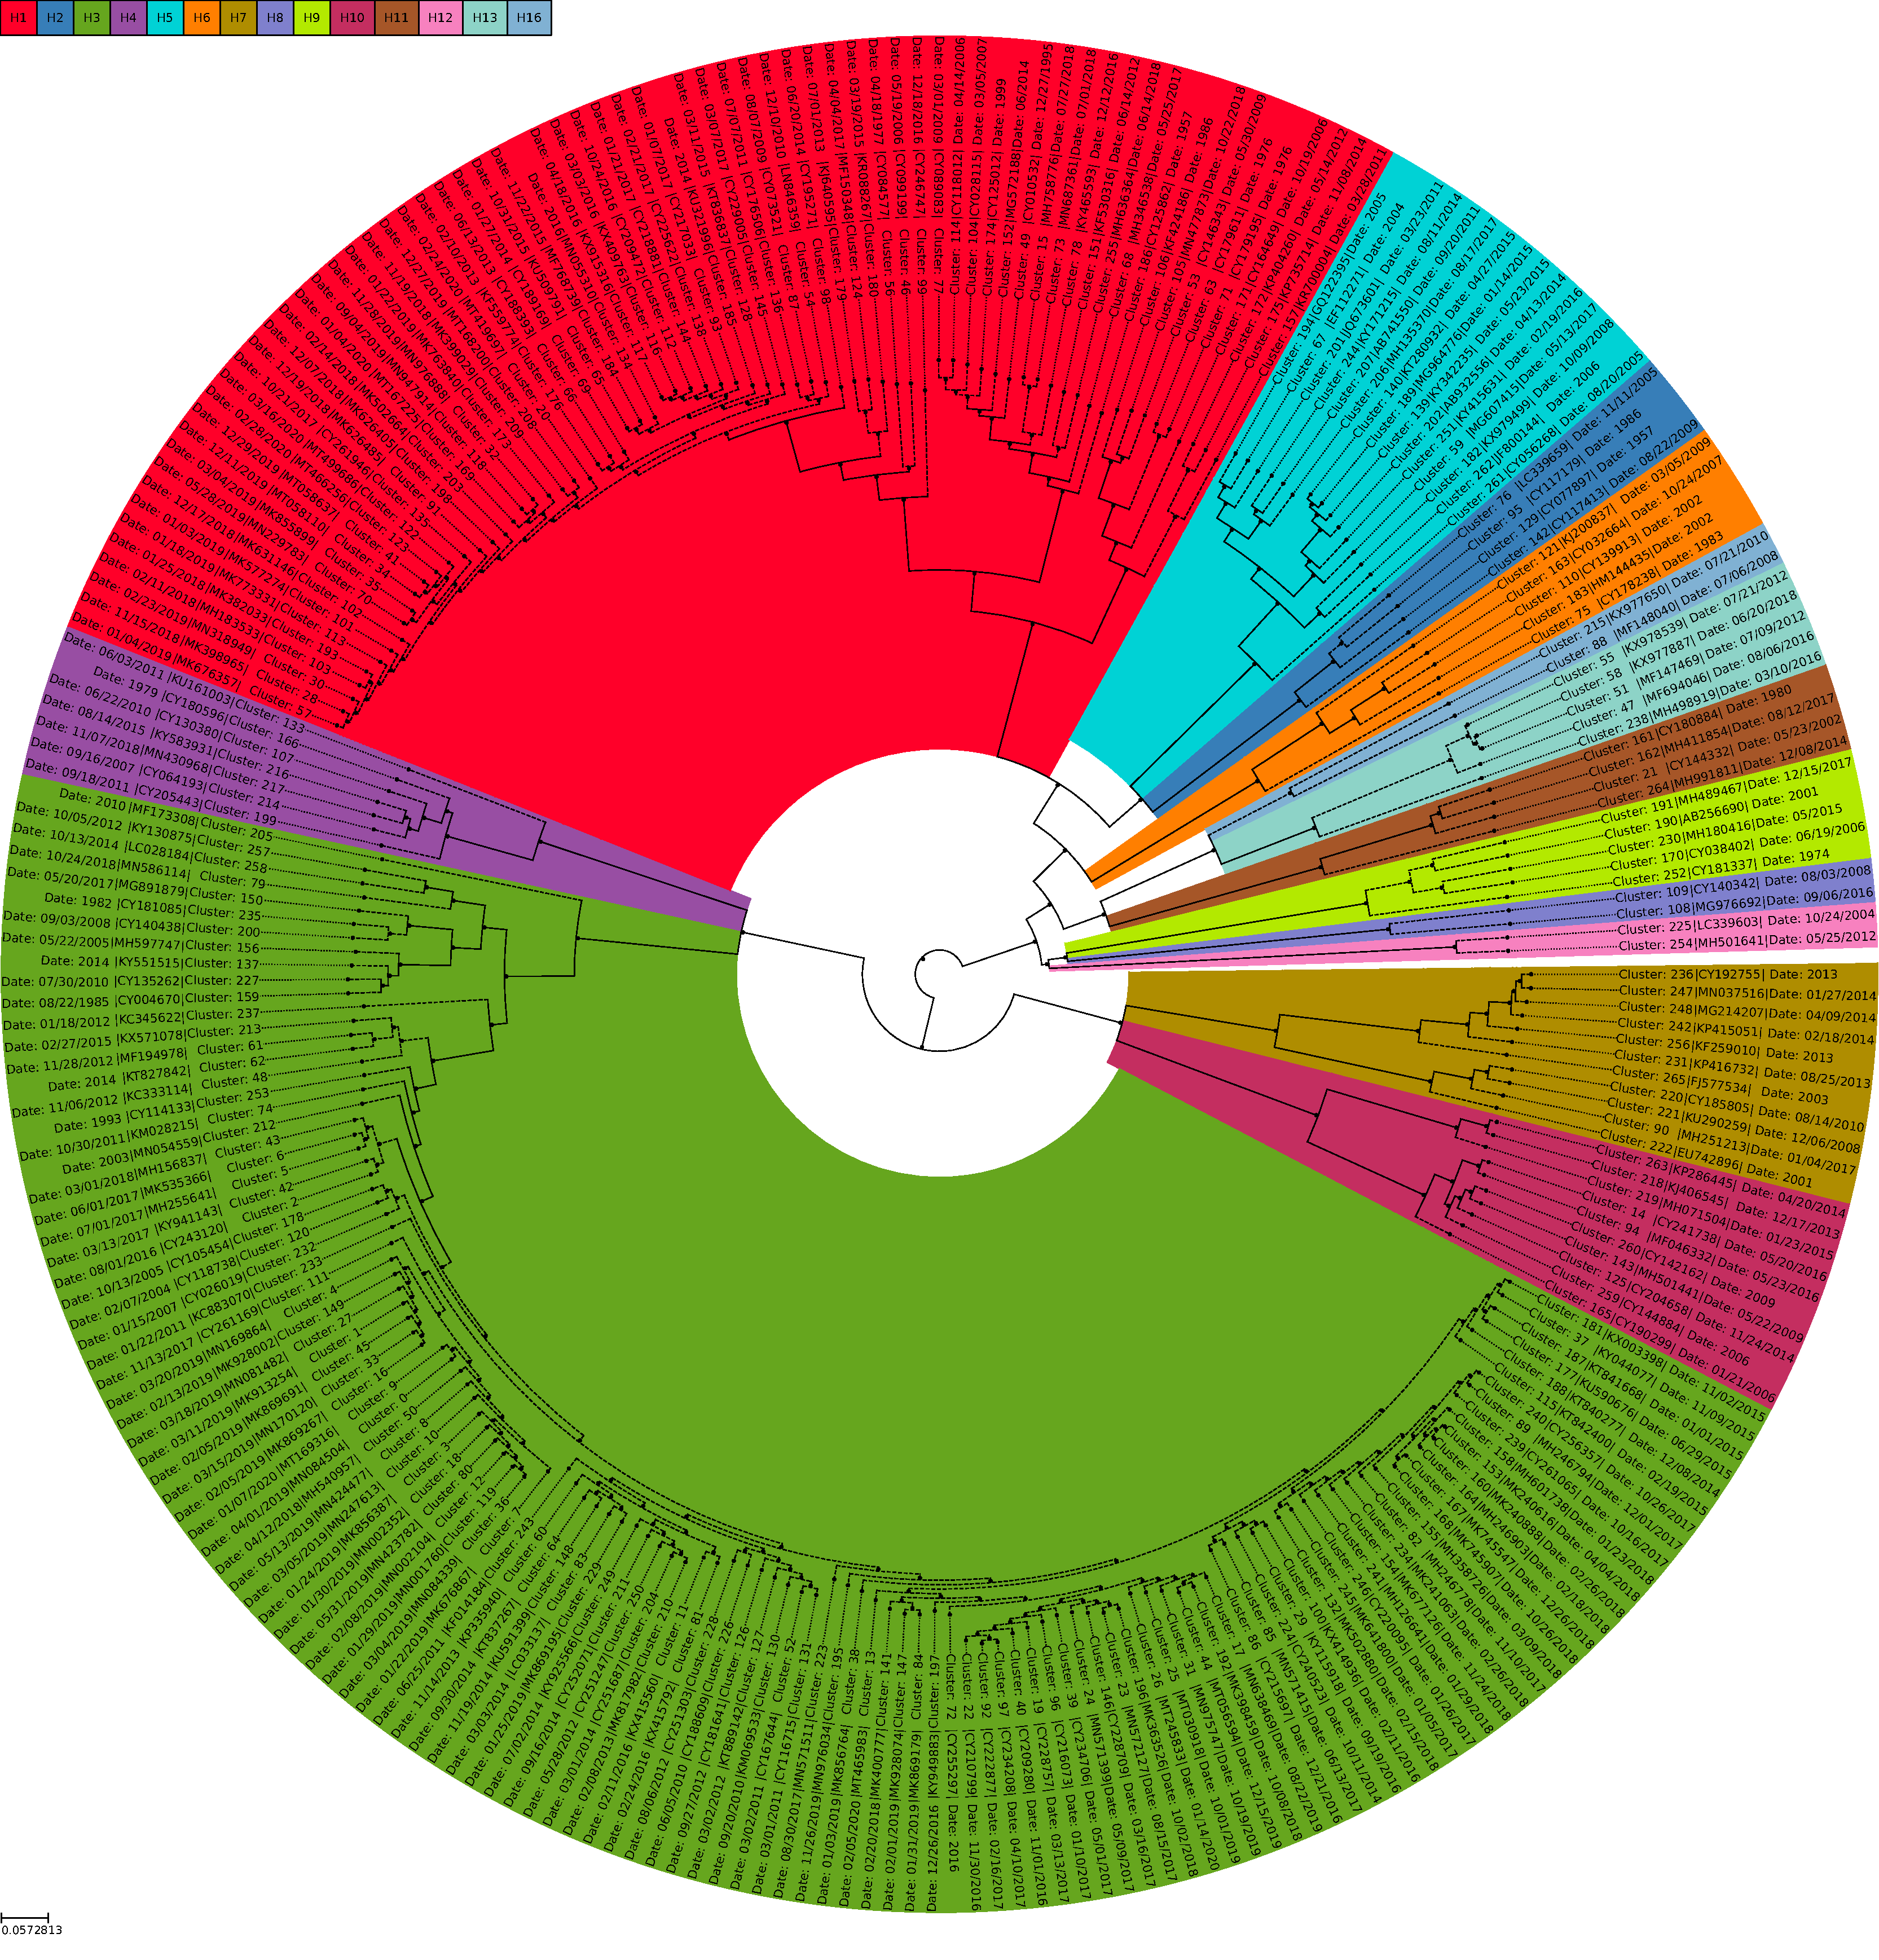
\includegraphics[width=\dimexpr\textwidth-2\fboxsep-2\fboxrule,fbox]{UMAP/Guidetree_segment_4_H_Centroid.pdf}
    \caption[Knee based Segment 4 Guidetree with \Acrshort{UMAP}]{\textbf{Knee based Segment 4 Guidetree with \Acrshort{UMAP}.} .}
    \label{fig:UMAP_Guidetree_Centroid_4}
\end{figure}

%Übergang zu cluster Comparison durch Centroid Alignment Tree -> H13/H16 Clustertree, Alignmenttree Vergleich -> Cluster H13/H16 Comparison